\chapter{Two Body Central Force Problems}
Here, we will explore the motion of two bodies that exert a conservative, central force on each other but are subject to no other, ``external" forces.      
\section{The Problem}
Consider two point particles with masses $m_1$ and $m_2$, with positions $\mbf r_1$, $\mbf r_2$ relative to some inertial frame. The only forces involved in the system are $\mbf F_{12}$ and $\mbf F_{21}$ of their mutual interaction. These forces can be derived from the potential energy $U(\mbf r_1, \mbf r_2)$ of their interaction. In the case of two astronomical bodies interacting through the gravitational force, the potential energy is
\[ U(\mbf r_1, \mbf r_2) = \frac{-Gm_1m_2}{\abs{\mbf r_1 - \mbf r_2}}\]
For two point charges interacting, the potential energy is
\[ U(\mbf r_1, \mbf r_2) = \frac{1}{4\pi\epsilon_0} \frac{q_1q_2}{\abs{\mbf r_1 - \mbf r_2}} \]
Note that in both of these examples, $U$ depends only on the difference $\mbf r_1 - \mbf r_2$, not on $\mbf r_1$ and $\mbf r_2$ separately. This is no accident, and it turns out that any isolated system is translationally invariant, and depends only on the difference between the positions. If a conservative force is central, then $U$ must also be independent of the direction of $\mbf r_1 - \mbf r_2$, and so it only depends on the magnitude $\abs{\mbf r_1 - \mbf r_2}$. 

It will be convenient to define a quantity known as the \textbf{relative position}, given by $\mbf r \equiv \mbf r_1 - \mbf r_2$. Then, we have
\[ U = U(\abs{\mbf r}) = U(r)\]
In terms of this new relative position, the Lagrangian becomes
\begin{align*}
    \L &= \frac{1}{2}m_1 \mbf{\dot r}_1^2 + \frac{1}{2}m_2 \mbf{\dot r}_2^2 - U(r)
\end{align*}
\section{Center of Mass and Relative Coordinates; Reduced Mass}
Our first task is to decide what generalized coordinate system to use. It seems natural to use the relative position $\mbf r$ as one of them, and it turns out that the other useful coordinate to use is the position of the center of mass $\mbf R = (m_1\mbf r_1 + m_2\mbf r_2)/(m_1+m_2)$.

As we know, the center of mass position lies on the line connecting them, with a distance along that line given by the ratio $\abs{\mbf R - \mbf r_2}/\abs{\mbf R - \mbf r_1} = m_1/m_2$. Further, we know that the momentum of the system is $\mbf P = (m_1+m_2)\mbf{\dot R}$, which implies that $\mbf{\dot R}$ is constant, by the conservation of momentum. This means that we can choose our (inertial) reference frame following the center of mass, so that $\mbf R$ is constant. 

We can write the coordinates of each mass in terms of the generalized coordinates $\mbf R$ and $\mbf r$ by noting
\begin{align*}
    \mbf r_1 &= \frac{m_1\mbf r_1 + m_2\mbf r_2}{m_1+m_2} + \frac{m_2}{m_1+m_2}(\mbf r_1 - \mbf r_2) \\
    &= \mbf R + \frac{m_2}{m_1+m_2}\mbf r = \mbf R + \frac{m_2}{M}\mbf r
    \intertext{and, through a similar analysis,}
    \mbf r_2 &= \mbf R - \frac{m_1}{m_1+m_2}\mbf r = \mbf R - \frac{m_1}{M}\mbf r
\end{align*}
This gives a Kinetic Energy of
\begin{align*}
    T &= \frac{1}{2}m_1 \pqty{\mbf{\dot R} + \frac{m_2}{m_1+m_2}\mbf{\dot r}}^2 + \frac{1}{2}m_2 \pqty{\mbf{\dot R} - \frac{m_1}{m_1+m_2}\mbf{\dot r}}^2 \\
    &= \frac{1}{2}(m_1+m_2)\mbf{\dot R}^2 + \frac{m_1m_2^2 + m_2m_1^2}{2(m_1+m_2)^2}\mbf{\dot r}^2 \\
    &= \frac{1}{2}(m_1+m_2)\mbf{\dot R}^2 + \frac{1}{2}\frac{m_1m_2}{m_1+m_2}\mbf{\dot r}^2
\end{align*}
By defining the total mass as $M = m_1 + m_2$, and a new quantity known as the \textbf{reduced mass} with $\mu = m_1m_2/M$, the kinetic energy becomes
\[ T = \frac{1}{2}M\mbf{\dot R}^2 + \frac{1}{2}\mu \mbf{\dot r}^2\]
This means that for all intents and purposes, the system is identical to a system with potential energy $U$ that involves a single particle of mass $M$ at the center of mass, and a fictitious particle of mass $\mu$ that moves with the speed of the relative position $\mbf r$.


With these simplifications, the Lagrangian becomes the sum of two independent components--one from the movement of the center of mass of the system, and one from the relative movement between the two particles.
\[ \L = \L_{\text{cm}} + \L_\text{rel} = \frac{1}{2}M\mbf{\dot R}^2 + \pqty{\frac{1}{2}\mu \mbf{\dot r}^2 - U(r)} \]
This means that we can solve for $\mbf R$ and $\mbf r$ in two entirely separate, uncoupled equations, which simplifies things greatly. 
\section{The Equations of Motion}
With the new Lagrangian, it is relatively easy to write the equations of motion for our particles. Because $\L$ is indepdent of $\mbf R$, $\mbf R$ is ignorable so the equation of motion is simply
\[ M\mbf{\ddot R} = 0\]
For $\mbf r$, each Euler-Lagrange equation gives
\[\mu {\ddot r_i} = -\pdv{U}{r_i}\]
or simply $\mu \mbf{\ddot r} = -\nabla U(\mbf r)$. In other words, the equation of motion for $\mbf r$ is identical to Newton's Second Law for a particle with mass $\mu$ and potential energy $U(r)$. 
\subsection*{The CM Frame}
Because $\mbf R$ is ignorable, we can choose a reference frame in which the center of mass is at rest--called the center of mass frame (CM frame). In this frame, $\mbf{\dot R} = 0$ and $\L_\text{CM} = 0$. Thus, in the CM frame,
\[ \L = \L_\text{rel} = \frac{1}{2}\mu \mbf{\dot r}^2 - U(r) \]
This justifies our terminology of the ``ignorable coordinate." By choosing a clever frame of reference, we literally can completely ignore the coordinate.

Using this frame of reference, our problem really is reduced to effectively being a one particle system, where the relative position $\mbf r$ can be thought of as the position of a particle of mass $\mu$ moving according to the potential energy function $U(r)$. 
\subsection*{Conservation of Angular Momentum}
We already know that the total angular momentum of our two particles is conserved. Like so many other things, angular momentum takes a quite simple form in the CM frame. In any frame, the total angular momentum is
\begin{align*}
    \mbf L &= \mbf r_1 \times \mbf p_1 + \mbf r_2 \times \mbf p_2 \\
    &= m_1 (\mbf r_1 \times \mbf{\dot r}_1) + m_2(\mbf r_2 \times \mbf{\dot r}_2)
\end{align*}
In the CM frame, we have $\mbf r_1 = (m_2/M) \mbf r$ and $\mbf r_2 = -(m_1/M) \mbf r$, so the angular momentum becomes
\begin{align*}
    \mbf L &= \frac{m_1m_2}{M^2} \pqty{m_2 \mbf r \times \mbf{\dot r} + m_1\mbf r \times \mbf{\dot r}} \\
    &= \mbf r \times \mu \mbf{\dot r}
\end{align*}
Notably, the angular momentum of the two particle system in the CM frame is exactly the same as it would be for a single particle with position $\mbf r$ and mass $\mu$. 

Perhaps the most remarkable part of this is that the conservation of angular momentum implies that $\mbf r \times \mbf{\dot r}$ is constant. In particular, its \textit{direction} is constant, which implies that the two vectors $\mbf r$ and $\mbf{\dot r}$ are constrained to one fixed plane, which we can take to be the $xy$ plane. In other words, the CM frame reduces the two body problem to a two dimensional problem. 
\subsection*{The Two Equations of Motion}
To set up the final equations of motion governing our two body system, lets first choose a set of generalized coordinates. The obvious choice is to pick the two dimensional polar coordinates within the plane of motion of the object. With this, the Lagrangian becomes
\[ \L = \frac{1}{2}\mu(\dot r^2 + r^2\dot\phi^2) - U(r)\]
since the Lagrangian is independent of $\phi$, the $\phi$ coordinate is ignorable and the Lagrange equation corresponding to $\phi$ is just
\[ \mu r^2\dot\phi = \text{constant} = \ell \]
since $\mu r^2 \dot\phi$ is the angular momentum $\ell$ (specifically, the $z$ component $\ell_z$), the $\phi$ equation is just a statement of conservation of angular momentum.

The $r$ equation (sometimes called the \textbf{radial equation}) is
\[ \mu \ddot r = \mu r\dot\phi^2 -\dv{U}{r} \]
If we move the $\mu r\dot\phi^2$ to the left, we obtain $\mu \ddot r - \mu r\dot\phi^2 = -\dd U/\dd r$, the radial component of $\mbf F = \mu \mbf a$. 
\section{The Equivalent One Dimensional Problem}
We can now work to solve the radial equation. One simplification we can do is to eliminate the variable $\dot\phi$ by writing $\dot\phi = \ell/(\mu r^2)$, giving us
\[ \mu \ddot r = -\dv{U}{r} + \frac{\ell^2}{\mu r^3} = -\dv{U}{r} + F_\text{cf} \]
which has the form of Newton's second law for a particle in one dimension with mass $\mu$ and position $r$, subject to the actual force $-\dd U/\dd r$ plus a ``ficticious" outward centrifugal force
\[ F_\text{cf} = \mu r \dot\phi^2 = \frac{\ell^2}{\mu r^3} \]
We can express the centrifugal force in terms of a centrifugal potential energy
\[ F_\text{cf} = -\dv{r} \frac{\ell^2}{2\mu r^2} = -\dv{U_\text{cf}}{r} \]
With this, the equation of motion becomes
\[ \mu \ddot r = -\dv{U}{r} - \dv{U_\text{cf}}{r} = -\dv{U_\text{eff}}{r} \]
where $U_\text{eff} = U + U_\text{cf}$ is the \textit{effective potential energy}.
\begin{example}[Effective Potential Energy for a Comet]
    Write down the actual and effective potential energies for a comet moving in the gravitational field in the sun, and use them to describe the motion.

    The actual gravitational potential energy of the comet is given by the well-known formula
    \[ U(r) = -\frac{Gm_1m_2}{r}\]
    The effective potential energy of this particle is equal to this \textit{plus} the centrifugal potential energy $\ell^2/(\mu r^3)$,
    \[ U_\text{eff}(r) = -\frac{Gm_1m_2}{r} + \frac{\ell^2}{2\mu r^2} \]
     \begin{minipage}{0.48\textwidth}
    when $r$ is large, the centrifugal potential energy term is negligible compared to the actual potential energy, and the effective potential energy is negative, sloping upward. When $r$ is small, assuming the angular momentum is nonzero, the centrifugal term dominates and the effective potential energy is positive, sloping downward.

   This implies that there will be a potential energy well when the effective potential energy stops decreasing and begins to increase, which causes oscillation between the potential and kinetic energy.
    \end{minipage}
    \begin{minipage}{0.48\textwidth}
    \parbox{\textwidth}{
        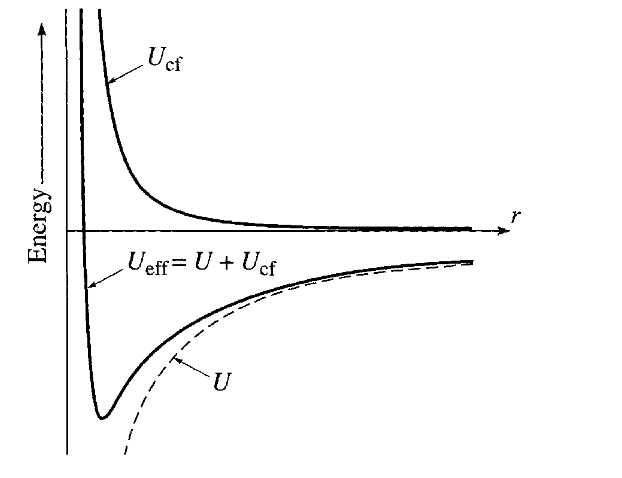
\includegraphics[width=0.8\textwidth]{effectivePE.png}
    }
    \end{minipage}
\end{example}
\subsection*{Conservation of Energy}
The derivative of the kinetic energy $T = \frac{1}{2}\mu \dot r^2$ is given by $\dot T = \mu \dot r \ddot r = -\dot r (\dd U_\text{eff}/\dd r) = -\dd U_\text{eff}/\dd t$. Or, in other words,
\[ \frac{\dd}{\dd t} \pqty{\frac{1}{2}\mu \dot r^2 + U_\text{eff}} = 0\]
Which is simply a statement of conservation of energy. If we write out $U_\text{eff}(r)$ as $U + \ell^2/(2\mu r^2)$ and replace $\ell$ with $\mu r^2\dot\phi$, we find
\[ \frac{1}{2}\mu \dot r^2 + U_\text{eff}(r) = \frac{1}{2}\mu \dot r^2 + \frac{1}{2}\mu r^2\dot\phi^2 + U(r) = E\]
This means that we can think of the total energy as simply the one dimensional kinetic energy of the radial motion, plus the effective one dimensional potential energy $U_\text{eff}$, since the latter includes the actual potential energy $U$ and the kinetic energy $\frac{1}{2}\mu r^2\dot\phi^2$. 